\chapter{Introduction}
\label{chapter:introduction}
Automated knowledge discovery methods are extremely important nowadays because of the 
amount of unstructured textual data. In order to utilise the information contained in the 
raw texts, one needs to find all the various objects mentioned there and find what kind of 
connections are between them according to the text. This is a quite demanding and 
time-consuming problem that requires experts' knowledge and skills. Thus the goal is to 
solve it by application of machine learning method, specifically Artificial Neural Network 
trained in a way that requires as less as possible experts' work.

\section{Motivation}
Knowledge Bases and Ontologies are crucial parts of any of expert system that are designed to
help professionals in their work. In order to obtain such a Knowledge Base, domain experts have to invest a lot of their costly time. They also have to curate the Knowledge Base over and over again because new knowledge is acquired and published continuously.

Usually, the subjects of interest are people, locations or organisations that are considered as 
\textit{entities}. Knowledge extraction is defined as the comprehension of the semantic meaning 
behind textual data, i.e. understanding which kinds of known relations connect entities.
Most common relations are binary, e.g. employee-of(person, organisation). If we think about 
more specific domains then entities might be genes, proteins, diseases for the biomedical domain, or 
algorithms, concepts and applications for the computer science domain and so on. Certainly, relational
classes can also become more specific.
 
Possible applications of the extracted knowledge are very diverse. One prototypical application is an expert 
system for collecting knowledge in the domain. For example in the Electronic Patient Path project, a system is aiming to help medical workers to find individual therapies for treating colorectal cancer. It has to contain a lot of knowledge about the field in order to give
adequate answers to given questions. Its core is a Knowledge Base containing all related entities 
and relations between them. Manipulation of such an up to date knowledge allows to quickly  
understand how to treat a new patient.

In order to better understand the idea behind Information Extraction, consider the following simple example.
\\\textit{''Interior Minister Giuliano Amato told lawmakers on Tuesday that more arrests were likely in Rome after police identify rioters. Holy Cross High School is a Catholic secondary school founded in Waterbury Connecticut in 1968 by the Congregation of Holy Cross. De La Salle High School was founded by the Christian Brothers. ''}
\\The text above contains several mentions of different people and organisations. Obviously, it should also contain 
 some information about their interactions. But just after reading the sentences time 
and effort are required to answer questions like:
\\\textit{''Who is Giuliano Amato? When and by whom was founded Hole Cross High School? Who founded De La Salle High School?''}
\\The task of information extraction is to simplify this process. Specifically, the process consists of 
finding entities or entity mentions:
\\\textit{''Interior Minister, Giuliano Amato, Rome; Holy Cross High School, Waterbuty, 1968, Congregation of Holy Cross; De La Salle High School, the Christian Brothers''}
\\and then interpreting the semantic meaning behind the text connecting these entities. Ideally, 
information extracted from this text will look like diagram depicted in the Figure 
\ref{fig:knowledge-graph}. Such kinds of diagrams can be seen as Knowledge Graphs and 
usually they are the most popular way of displaying content of a Knowledge Base. Having such 
a Knowledge Base answering aforementioned questions might be completely 
automatised thus requiring no human effort. It should be noticed, that 
sometimes the text will not contain enough information to name the exact relation between 
some of the marked entities. For example, the considered sentence does not contain any exact relation
between \textit{Giuliano Amato} and \textit{Rome}. This is important, as marking all 
the known entities in the textual data will create a lot of noise that should be somehow 
filtered during the Relation Extraction process.

	\begin{figure}
		\centering
		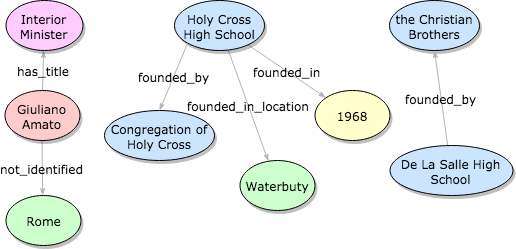
\includegraphics[width=0.8\linewidth]{chapter1_introduction/images/knowledge-graph}
		\caption[Example of Knowledge Graph]{Knowledge extracted from textual data in the form of Knowledge Graph.}
		\label{fig:knowledge-graph}
	\end{figure}

For now, the creation of
a Knowledge Base is still a problem that requires experts work. Automated methods currently suffer 
from many pitfalls, e.g exploiting pipelines of Natural Language Processing tools which are not always 
accurate and introduces its own miscalculations that lead to the higher overall error rate. Another 
challenge is the necessity of training examples for most of the machine learning models. There 
usually does not exist sufficient amount of labeled examples of 
relations in natural texts because labelling texts is a very time-consuming and 
effort demanding activity. 

Nevertheless, there is a huge volume of raw textual data and some already created and curated 
Knowledge Bases that definitely can be very helpful in solving the problem of Information Extraction. 
The process of knowledge discovery might be improved and all existing structured and 
unstructured data should be exploited for it.

\section{Goals}
The main idea in this work is to explore the ways in which deep-learning can be 
used for solving the problem of Relation Extraction and Classification. This research
plans to tackle this problem in general and for the medical domain in particular. 

The goal is to improve Relation Extraction by usage of Deep Learning methods together with 
weak supervision and Multiple Instance Learning. The chosen approach is to
apply the Convolutional Neural Network proposed in 
\cite{DBLP:journals/corr/SantosXZ15} combined with Distant Supervision \cite{Mintz:2009:DSR:1690219.1690287} 
and Multiple Instance Learning \cite{zeng2015distant}. The idea behind is that a Convolutional Neural Network 
should be able to identify critical parts of a sentence and transform them to a feature vector 
that can be identified as belonging to one or other relation. The concept of the Distant Supervision 
aims to remove the need of manually labeled examples or at least limit the needed amount. It 
exploits the knowledge contained in the existing sources of structured data and makes use of 
raw unstructured texts aligning them together for getting training datasets. As it suffers from 
very general assumption that 
\\'\textit{'Every sentence containing two related entities will describe this 
relation'' }
\\a lot of methods for improving it were studied. One of them is Multiple Instance Learning 
that mitigates the assumption by giving a label not to one sentence, but to the set or so-called 
bag of sentences with the same entities pair and saying that at least one of them should describe this 
relation. 

One of the questions that can be answered is how Distant Supervision affects the Relation Extraction problem
 solved with Convolutional Neural Network. It is important to understand how and where experts 
should be involved in order to obtain a maximal result with minimal effort and time. 

\section{Structure of the thesis}
Experiments are aimed to answer questions about the helpfulness of the Distant Supervision approach 
and the possibilities to improve knowledge discovery with minimally manned methods. Any textual 
information available can be considered as a source of examples for the general domain and there 
exist various public Knowledge Bases. As it is easier to validate the result in general domain than in 
specific medical one, the first part of experiments are performed for general domain data and then 
the model is applied to the medical domain. For the medical domain a large volume of raw texts from PubMed \footnote{\url{https://www.ncbi.nlm.nih.gov/pubmed}} 
along with existing medical Knowledge Base and ontologies is used.

The structure of the text is following:
\begin{itemize}
  \item Chapter \ref{chapter:background} describes the background knowledge about the 
  problem of Natural Language Processing, Relation Extraction and lists relevant approaches
  \item Chapter \ref{chapter:approach} specifies the exact approach chosen for this thesis 
  and describes various implementation details
  \item Chapter \ref{chapter:experiments} shows evaluation results on different datasets in 
  different domains
  \item Chapter \ref{chapter:conclusion} suggests future work and observations made during 
  performing the evaluation of the approach
\end{itemize}
